 % Tarea 1 ED
 

\section{Bitácoras}

\subsection{Bitácora 1}
Se inicio con una compuerta XOR en \textit{TinkerCad} la cual me dio problemas por el hecho de que no concuerda con la tabla de verdad, cada una de las entradas se hicieron con un pull up y un pull down respectivamente.

\subsection{Bitácora 2}
Se arreglo el error en la entrada del pull up, el LED está encendido sin necesidad de presionar el push button. La tabla de verdad para XOR y la tabla de verdad obtendida con el circuito es:

\begin{table}[H]
	\centering
	\caption{Tabla de datos obtenida por el circuito \ref{XORi}. (XOR)}
	\label{XOR}
	\begin{tabular}{||c|c||c|c||}
		\hline
		\hline
		\multicolumn{2}{||c||}{INPUT} & EXPECTED OUTPUT & RESULT OUTPUT \\
		\hline
		\hline
		$0$ & $0$ & $0$ & $0$ \\
		$0$ & $1$ & $1$ & $0$ \\
		$1$ & $0$ & $1$ & $1$ \\		
		$1$ & $1$ & $0$ & $0$ \\
		\hline
		\hline
	\end{tabular}
\end{table}

\begin{figure}[H]
	\centering
	\label{XORi}
	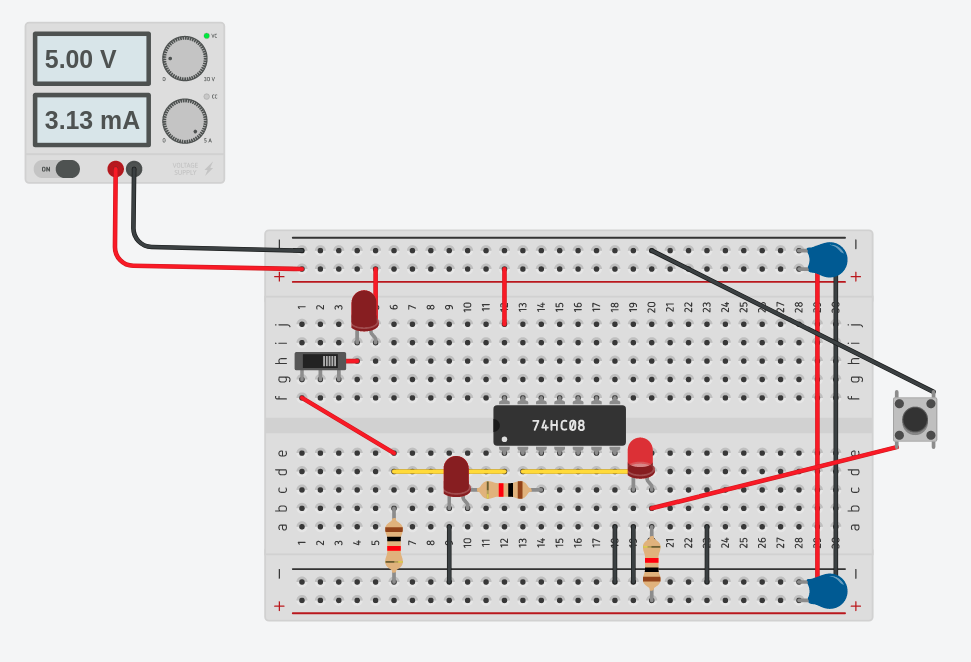
\includegraphics[scale=0.25]{Images/XOR.png}
	\caption{Circuito que modela la operación binaria XOR.}
\end{figure}


\subsection{Bitácora 3}

Se realizo la compuerta AND, también con una entrada pull up y una pull down. Con esto, en la pull up, se tenía problemas con el LED, así que se obvio dicho LED y se hicieron las respectivas pruebas. Lo cual resultó en la compuerta deseada:

\begin{figure}[H]
	\centering
	\label{ANDi}
	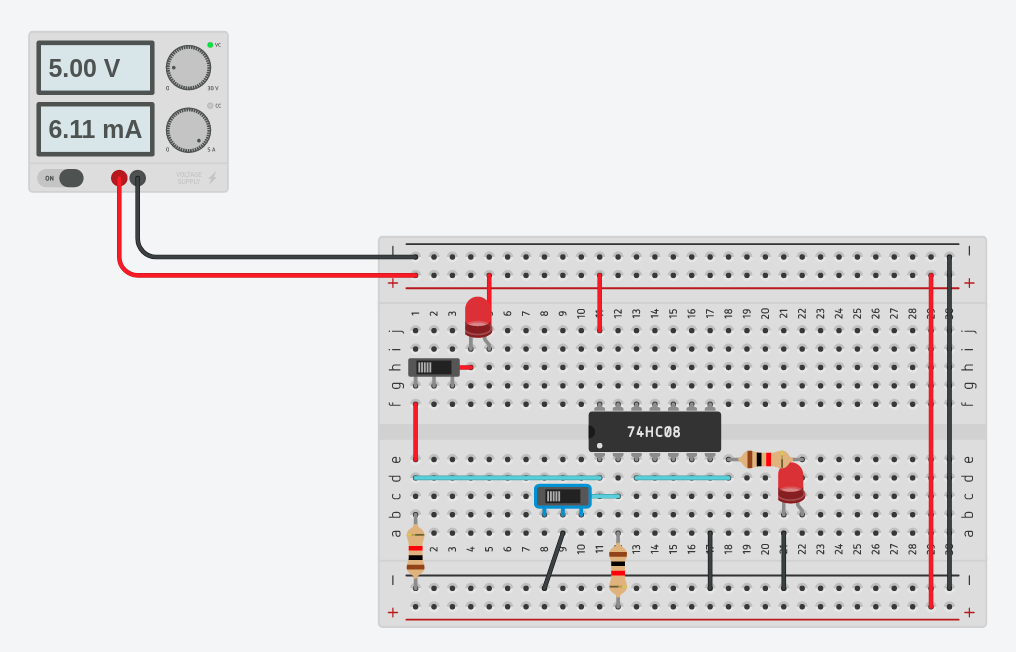
\includegraphics[scale=0.4]{Images/AND.png}
	\caption{Circuito de compuerta AND con entradas pull up y pull down.}
\end{figure}


\begin{table}[H]
	\centering
	\caption{Tabla de datos obtenida por el circuito \ref{ANDi}. (AND)}
	\label{XOR}
	\begin{tabular}{||c|c||c|c||}
		\hline
		\hline
		\multicolumn{2}{||c||}{INPUT} & EXPECTED OUTPUT & RESULT OUTPUT \\
		\hline
		\hline
		$0$ & $0$ & $0$ & $0$ \\
		$0$ & $1$ & $0$ & $0$ \\
		$1$ & $0$ & $0$ & $0$ \\		
		$1$ & $1$ & $1$ & $1$ \\
		\hline
		\hline
	\end{tabular}
\end{table}












































